\section{符号函数}
\begin{definition}[符号函数]
函数\begin{equation*}
	f(x) = \left\{ \begin{array}{cc}
		1, & x > 0 \\
		0, & x = 0 \\
		-1, & x < 0 \\
	\end{array} \right.
\end{equation*}称为\DefineConcept{符号函数},
记作\(\sgn x\).
\end{definition}

\begin{figure}[htb]
	\centering
	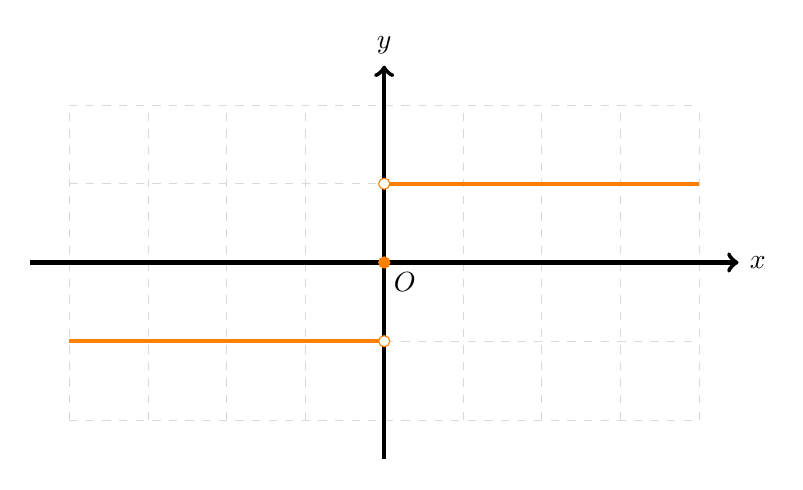
\begin{tikzpicture}
		\draw[help lines, color=gray!30, dashed] (-4,-2) grid (4,2);
		\draw[->, ultra thick] (-4.5,0) -- (4.5,0) node[right]{\(x\)};
		\draw[->, ultra thick] (0,-2.5) -- (0,2.5) node[above]{\(y\)};
		\draw (0,0)node[below right]{\(O\)};
		\draw[orange,ultra thick] (-4,-1)--(0,-1) (0,1)--(4,1);
		\draw[draw=orange,fill=orange] (0,0)circle(2pt);
		\draw[draw=orange,fill=white] (0,1)circle(2pt) (0,-1)circle(2pt);
	\end{tikzpicture}
	\caption{符号函数\(\sgn x\)的图形}
\end{figure}
